\documentclass[10pt]{article}
\usepackage{icmlko}

\icmlmeta{IP 파운데이션 월드모델}{221}{덮음을 올렸더니 축이 뒤집혔다}{여든 노트 넘게 ``제목 언어 한계''로 적혀 있던 것이 문자열 버그였다. 고쳐서 채웠더니 새로 덮인 곳의 축이 반대로 움직인다}

\begin{document}

\twocolumn[
\icmlheader

\begin{abstract}
노트 220이 검색 무리의 천장을 $+$0.0365 로 재고 ``게임 · 모바일 덮음을
채우면 값이 있다''를 남겼다. 열었더니 \textbf{언어 한계가 아니라 문자열
버그였다.} \texttt{ingest/trend\_all.py} 의 \texttt{clean\_kw} 가
\texttt{re.split(...)[0]} 로 앞 조각만 썼는데, ① ``Palworld / 팰월드''는
영문 쪽을 집고 한글 쪽을 버려 한글 문턱에 걸려 통째로 빠지고, ②
``(자막) 도굴왕''처럼 괄호로 시작하면 첫 조각이 \emph{빈 문자열}이라
역시 빠진다. \textbf{②가 크다 --- 애니 2,073건 중 486건}이다. 고치니
대상이 5,959 $\to$ \textbf{6,595}(애니 $+$486 · 모바일 $+$81 · 펀딩
$+$53 · 게임 $+$9)이고, 데이터랩에서 채우니 덮음이 \textbf{애니 82.5\%
$\to$ 98.5\% · 펀딩 86.2\% $\to$ 100\% · 모바일 54.2\% $\to$ 60.1\% ·
게임 36.7\% $\to$ 40.6\%} 로 올랐다. \textbf{그런데 판이 갈라진다} ---
능형이 $+$0.4288 $\to$ $+$0.4195, F21 이 $+$0.4395 $\to$ $+$0.4321 로
내리고 \textbf{배깅 트리만 $+$0.4396 $\to$ $+$0.4523 으로 오른다.}
갈랐다. \textbf{새로 덮인 행의 축이 반대로 움직인다} --- 애니에서 옛
덮음 500건은 수준 $+$0.057 · 모멘텀 $+$0.194 · 변동 $+$0.064 인데
\textbf{새 덮음 97건은 $-$0.191 · $-$0.082 · $-$0.234} 다. 모바일도
$+$0.320 $\to$ $+$0.088 로 사분의 일이다. 까닭을 \textbf{라벨을 한 번도
안 보고} 찾았다 --- 새 키워드는 \textbf{계열 질의}다. 제목 셋 이상에
등장하는 키워드 비중이 애니에서 옛 10.3\% 대 \textbf{새 29.6\%} 이고,
키워드가 원 제목에서 차지하는 길이 비의 중앙이 \textbf{1.00 대 0.58} 이다.
``(자막) 블리치-천년혈전 편 : 화진담''에서 뽑은 ``블리치-천년혈전 편''은
그 회차가 아니라 \emph{계열}을 재는 질의다. 무효는 아니고 \textbf{더 거친
측정}이다 --- 그래서 지우지 않고 모형에게 구분할 수단을 줬다. 계열 질의
표시자를 얹으니 능형이 $+$0.4195 $\to$ $+$0.4241 로 \textbf{잃은 것의
절반}을 되찾는다(트리는 $-$0.0009). \textbf{교훈은 덮음이 곧 개선이
아니라는 것이다} --- 같은 열 이름 아래 다른 것을 재는 값이 들어오면,
트리는 그것을 갈라 쓰고 능형은 못 쓴다.
\end{abstract}
]

\begin{figure*}[t]
\centering
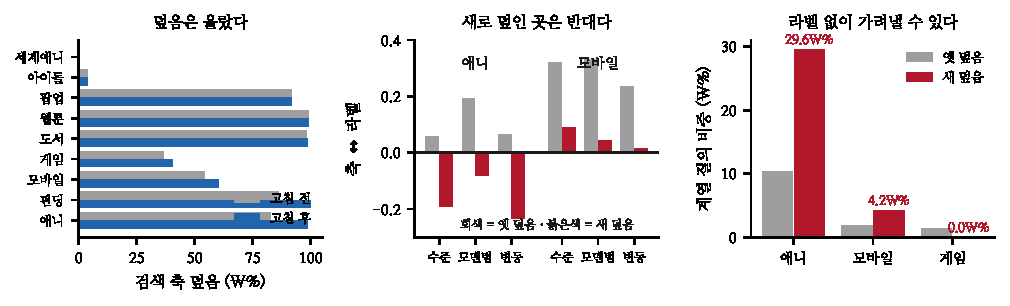
\includegraphics[width=\textwidth]{figs/broadq.pdf}
\caption{왼쪽 --- 덮음은 올랐다. 가운데 --- 새로 덮인 곳은 부호가 반대다.
오른쪽 --- 라벨 없이 가려낼 수 있다.}
\end{figure*}

\section{언어 한계가 아니라 문자열 버그였다}

\claimx{\texttt{clean\_kw} 가 \texttt{re.split(...)[0]} 로 앞 조각만 썼다.
``(자막) 도굴왕''은 첫 조각이 \emph{빈 문자열}이라 통째로 빠진다 ---
\textbf{애니 2,073건 중 486건이 이것이다.}}{여든 노트 넘게 열린 갈래
목록에 ``제목 언어 한계''로 적혀 있었다. \textbf{노트 219가 ``갈래 목록은
삭는다''고 했는데, 삭는 것만이 아니라 \emph{처음부터 틀린} 것도 있었다.}}

\begin{table}[t]
\centering\tsize
\caption{고침 뒤 대상 수와 유보 덮음.}
\begin{tabular}{lrrrr}
\toprule
& 대상 전 & 대상 후 & 덮음 전 & 덮음 후 \\
\midrule
\textbf{애니} & 1{,}547 & \textbf{2{,}033} & 82.5\% & \textbf{98.5\%} \\
모바일 & 824 & 905 & 54.2\% & 60.1\% \\
\textbf{펀딩} & 345 & 398 & 86.2\% & \textbf{100\%} \\
게임 & 147 & 156 & 36.7\% & 40.6\% \\
웹툰 & 2{,}749 & 2{,}755 & 98.9\% & 99.0\% \\
\bottomrule
\end{tabular}
\end{table}

\claimx{\textbf{앞머리를 무조건 떼는 판을 만들었다가 되돌렸다} --- 애니는
``(자막) 제목''이라 앞이 꼬리표인데 \emph{펀딩은} ``[제목] 설명''이라
앞이 제목이다.}{위치가 아니라 \textbf{꼬리표 목록}으로 거른다. 재 보고
알았다 --- 안 재고 고쳤으면 펀딩을 망가뜨렸을 것이다.}

\section{판이 갈라진다}

\begin{table}[t]
\centering\tsize
\caption{판 $\rho$.}
\begin{tabular}{lrrr}
\toprule
& 고침 전 & 고침 후 & $+$계열 표시자 \\
\midrule
F6 능형 & \textbf{.4288} & .4195 & .4241 \\
F21 & \textbf{.4395} & .4321 & .4324 \\
\textbf{F18 배깅} & .4396 & \textbf{.4523} & .4514 \\
\bottomrule
\end{tabular}
\end{table}

\claimx{\textbf{선형 둘은 내리고 트리만 오른다.} 챔피언이 다시 F18 로
넘어간다($+$0.4523).}{\textbf{자료를 더 채웠는데 절반이 나빠지면 채운
것이 같은 것이 아니다} --- 노트 207 · 210 · 213의 모양이다.}

\section{새로 덮인 곳은 반대다}

\begin{table}[t]
\centering\tsize
\caption{유보에서 축 $\leftrightarrow$ 라벨.}
\begin{tabular}{llrrr}
\toprule
& & 수준 & 모멘텀 & 변동 \\
\midrule
\textbf{애니} & 옛 덮음(500) & $+$.057 & $+$.194 & $+$.064 \\
& \textbf{새 덮음(97)} & \textbf{$-$.191} & \textbf{$-$.082} & \textbf{$-$.234} \\
\midrule
모바일 & 옛 덮음(239) & $+$.320 & $+$.332 & $+$.236 \\
& 새 덮음(26) & $+$.088 & $+$.043 & $+$.015 \\
\bottomrule
\end{tabular}
\end{table}

\claimx{\textbf{애니는 부호가 뒤집히고 모바일은 사분의 일이 된다.}
같은 열 이름 아래 다른 것이 들어왔다.}{\textbf{그리고 그것이 판이
갈라진 까닭이다} --- 트리는 부분집단을 갈라 쓸 수 있고 풀링 능형은
계수 하나를 쓰므로 상쇄를 그대로 먹는다(노트 186의 부호 이질성과 같은
기전).}

\section{라벨 없이 가려낼 수 있다}

\begin{table}[t]
\centering\tsize
\caption{키워드가 작품 질의인가 계열 질의인가.}
\begin{tabular}{llrr}
\toprule
& & 계열 질의 & 길이 비 \\
\midrule
\textbf{애니} & 옛 덮음 & 10.3\% & 1.00 \\
& \textbf{새 덮음} & \textbf{29.6\%} & \textbf{0.58} \\
모바일 & 옛 덮음 & 1.8\% & 1.00 \\
& 새 덮음 & 4.2\% & 0.38 \\
\bottomrule
\end{tabular}
\end{table}

\claimx{\textbf{새 키워드는 계열 질의다} --- 제목 셋 이상에 등장하는
비중이 세 배이고, 키워드가 원 제목에서 차지하는 길이 비의 중앙이
1.00 에서 0.58 로 떨어진다.}{``(자막) 블리치-천년혈전 편 : 화진담''에서
뽑은 ``블리치-천년혈전 편''은 그 회차가 아니라 \emph{계열}을 재는
질의다. \textbf{제목과 키워드만으로 판정되므로 라벨을 안 본다.}}

\claimx{\textbf{무효가 아니라 더 거친 측정이다.} 계열 검색량은 실재하고
예측력도 있다 --- 다만 계열 안에서는 회차를 못 가른다.}{그래서 지우지
않는다. 노트 213(공휴일 목록 밖)과 다르다 --- 거기는 값이 \emph{정의}
되지 않았고 여기는 정의되되 \emph{거칠다}.}

\begin{table}[t]
\centering\tsize
\caption{계열 질의 표시자를 얹으면.}
\begin{tabular}{lrrr}
\toprule
& 그대로 & 표시자 & 차 \\
\midrule
\textbf{F6 능형} & .4195 & \textbf{.4241} & \textbf{$+$.0046} \\
F21 & .4321 & .4324 & $+$.0003 \\
F18 배깅 & .4523 & .4514 & $-$.0009 \\
\bottomrule
\end{tabular}
\end{table}

\claimx{\textbf{능형이 잃은 것($-$0.0093)의 절반을 되찾는다.} 트리는
$-$0.0009 로 안 움직인다 --- \textbf{이미 그 구분을 스스로 하고
있었다.}}{노트 218과 같은 모양이고 결과도 같다 --- \textbf{능형에게
없는 것을 명시로 주면 일부는 메워지고 트리는 안 움직인다.} 다만
절반만 메워지므로 \textbf{트리는 이 표시자가 표현하는 것보다 더 세밀한
구분을 하고 있다.}}

\begin{table}[t]
\centering\tsize
\caption{남은 것.}
\begin{tabular}{ll}
\toprule
\textbf{계열 질의} & 계열 안 순위를 다른 축으로 가를 수 있나 \\
\textbf{게임 영문} & 322건 --- 음역하면 덮음 41\%$\to$? \\
채택 판단 & 트리 우위가 이질성 이용인지 다시 볼 것 \\
\bottomrule
\end{tabular}
\end{table}

셋째 줄이 다음 사이클의 첫 칸이다. \textbf{이 사이클에서 챔피언이 두 번
바뀌었다} --- 노트 215가 공휴일을 고쳐 트리에서 F21 로 넘겼고, 이 노트가
검색을 채워 다시 트리로 돌렸다. \textbf{두 번 다 자료를 고친 결과이고
모형을 손댄 것이 아니다.} 그런데 이번 트리 우위($+$0.0202)는
\textbf{축의 이질성을 가르는 데서 온다} --- 노트 214가 잡은 ``학습 전용
스위치''와는 다르지만, \emph{모형이 자료의 결함을 이용해 이긴다}는
점에서 같은 계열이다. \textbf{그 우위가 이질성을 지우면 사라지는지}를
재야 챔피언을 확정할 수 있다.

\end{document}
